\section{Auswahl einer Drohne}
\label{drone_selection}

Bei der Auswahl der Drohne sind vor allem zwei Bereiche zu betrachten:

\begin{itemize}
	\item Die gesetzlichen Rahmenbedingungen zur Drohne und
	\item Die technischen Anforderungen an die Drohne.
\end{itemize}

Was die gesetzlichen Anforderungen betrifft, so wurden im Juni 2019 von der \textit{European Aviation Safety Agency} (EASA) einheitliche Regeln veröffentlicht, die den Drohnenbetrieb in der Europäischen Union einheitlich regeln sollen. Da den Mitgliedsstaaten ein Zeitraum von einem Jahr zur Umsetzung der Regularien zugesprochen wurde, gelten in Deutschland weiterhin die Vorschriften der deutschen Drohnen-Verordnung von 2017 \cite{EASA.2019}.

Diese schreiben unter anderem vor \cite{Drohnen.de.2020}:
\begin{itemize}
	\item Eine Kennzeichnungspflicht ab einem Startgewicht von über 250g,
	\item Eine maximale Flughöhe von 100 Metern über dem Grund,
	\item Eine Haftpflichtversicherung und
	\item Flugverbotszonen (Wohngrundstücke, Naturschutzgebiete, etc.).
\end{itemize}

Aufgrund dieser Auflagen wurde der Beschluss gefasst, dass die auszuwählende Drohne nur innerhalb von geschlossenen Wohnräumen im privaten Betrieb genutzt werden soll und zudem ein Startgewicht von unter 250g besitzen soll. Um eine studentische Machbarkeitsstudie durchführen zu können, ist eine solche eingeschränkte Anwendungsumgebung allemal ausreichend. 

Die Programmierbarkeit der Drohne gehört zu der wichtigsten technischen Anforderung an die Drohne. Zudem soll sie eine integrierte Kamera aufweisen, die in der Lage ist, einen Videostream zur Laufzeit zur Verarbeitung bereit zu stellen. Auch die Akkulaufzeit und Robustheit der Drohne wurden als Entscheidungskriterien aufgenommen. Bezüglich der Kostenübernahme konnte zuvor eine Einigung mit Vertretern des Informatik Labors der DHBW Karlsruhe erzielt werden. Die Kosten werden vollständig übernommen, solange sie sich im Rahmen eines Studienarbeit angemessenen Budgets befinden.

Die sehr speziellen Anforderungen ließen nur ein Drohnen Modell auf dem Markt zu, die \textit{Tello EDU} Drohne von der Firma Ryze Tech. Sie bietet eine Kamera mit 720p Übertragungsqualität an, eine Akkulaufzeit von 13 Minuten und eine Programmierschnittstelle für die Steuerung sowie das Empfangen von Aufzeichnungen der Kamera. Auch wirbt sie mit der Fähigkeit von präzisem Schweben, was gerade für die Objektdetektion von Vorteil sein könnte \cite{RyzeRobotics.2020}.

Für die Steuerung sowie den Zugriff auf den Videostream bietet die \textit{Tello EDU} ein eigenes WiFi Netz an, zu dem sich das Steuergerät verbinden muss. Die Kommunikation erfolgt über das \textit{UDP} Protokoll\footnote{UDP steht für User Datagram Protocol. Es ist ein Transportprotokoll, welches im Gegensatz zu TCP verbindungslos und nicht zuverlässig ist.} und besteht aus mehreren Kommunikationskanälen: 

\begin{figure}[H]
	\begin{center}
		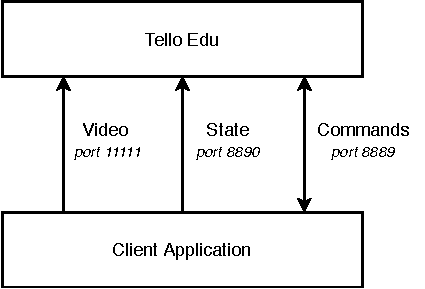
\includegraphics[width=8cm]{Bilder/communication_tello.pdf} 
		\caption{Kommunikationskanäle der Tello Edu Drohne}
		\label{communication_tello}
	\end{center}
\end{figure}

Der Video Stream und der Status der Tello Edu werden unidirektional durch die Client Applikation bei der Tello Edu abgefragt, wohingegen für das Senden von Befehlen eine bidirektionale Verbindung zum Einsatz kommt. Das liegt daran, dass die Tello Edu auf jeden erhaltenen Befehl auch eine Antwort zurücksendet. Es existieren Befehle zur Steuerung und zum Auslesen von Informationen wie zum Beispiel der Geschwindigkeit oder Ladezustand der Batterie. Als Hilfestellung wird zusätzlich ein Beispielprogramm mitgeliefert, in welchem das Senden und Empfangen von Befehlen implementiert wurde \cite{RyzeTech.2018}. 